\documentclass[10pt,a4paper]{report}
\usepackage[latin1]{inputenc}
\usepackage[dutch]{babel}
\usepackage{amsthm}
\usepackage{amsmath}
\usepackage{amssymb}
\usepackage{graphicx}
\usepackage{pdfpages}
\usepackage{wrapfig}

\makeatletter
\renewcommand{\@makechapterhead}[1]{%
\vspace*{50 pt}%
{\setlength{\parindent}{0pt} \raggedright \normalfont
\bfseries\Huge Vraag \thechapter :\;#1
\par\nobreak\vspace{20 pt}}}
\makeatother

\title{Algoritmen en Datastructuren\\ Taak 1: het Collections Framework}
\author{Tom Naessens\\ Academiejaar 2010 -- 2011}

\parindent 0pt
\begin{document}
\maketitle

%%%%%%%%%%%%%%%%%%%%%%%%%%%%%%%%%%%%%%%%%
%%%%			VRAAG 1                 %%%%
%%%%%%%%%%%%%%%%%%%%%%%%%%%%%%%%%%%%%%%%%

\section*{Vraag 1: Gegevens verwijderen}
\subsection*{Gebruikte datastructuren en algoritmen}
\subsubsection*{Gebruikte datastructuren}
Voor deze klasse heb ik, zoals de opdracht vermeldde, gebruik gemaakt van een ArrayList en van een LinkedList. Beiden werden ze aangemaakt bovenaan de klasse. Deze lijsten hadden als type 'NormalPerson'. De lijsten werden ge\"instantieerd in de constructor van de klasse. In de methode \textsl{addPerson()} kan door middel van de \textsl{add()} methode een persoon aan de klasse toegevoegd worden.
\subsubsection*{Gebruikte algoritmen}
Het algoritme is dezelfde voor zowel de ArrayList als de LinkedList. De lijst wordt doorlopen met een iterator tot het einde van de lijst. Omdat je een lijst niet mag wijzigen terwijl je ze overloopt maak ik in deze methode gebruik van een Iterator. Ik overloop de lijst van begin tot einde omdat het zou kunnen dat op de laatste plaats toch nog een persoon staat die verwijdert moet worden. Voortijdig stoppen kan dus niet. Iedere keer ik een persoon tegenkom van wie de gemeente overeen komt met de opgegeven plaats verwijder ik deze en voeg ik zijn ID toe aan een lijst. Op het eind van deze methode retourneer ik de lijst met ID's.\\

De complexiteit van de functies verschillen echter wel. 
Bij een ArrayList is de complexiteit van de functie $\theta(n^2)$. 
Bij het overlopen van de lijst van personen hebben we een complexiteit van $\theta(n)$ maar door de verwijderbewerking komt hier nog een $\theta(n)$ bij aangezien de ArrayList de vrijkomende plaats moet opvullen.\\
Een LinkedList geeft ons immers een complexiteit van $\theta(n)$. Het overlopen van de lijst geeft ons $\theta(n)$ en het verwijderen uit een LinkedList is constant, $\theta(1)$ dus.
\subsection*{Tijdsmetingen}
\subsubsection*{Grafieken}
Voor deze en volgende klasses te testen heb ik de volgende werkwijze gehanteerd:\\
Om ervoor te zorgen dat ik een betrouwbaar overzicht kreeg heb ik iedere keer in een testklasse mijn methodes getest. Ik begon steeds bij inputwaarden lager dan 100.000 en verhoogde deze steeds met 50.000. Voor elke inputwaarde herhaalde ik de test 10 keer en nam het gemiddelde van deze 10 tests als uitvoeringswaarde. Iedere keer nadat ik een object van mijn klasse aanmaakte verwijderde ik dit object en riep ik \textsl{System.gc()} aan om er zeker van te zijn dat er geen oude data in het geheugen bleef zitten. Waar de trendlijn een goed beeld van de functie gaf liet ik een trendlijn tekenen.
\begin{figure}[h!]
    \centering
    \fbox{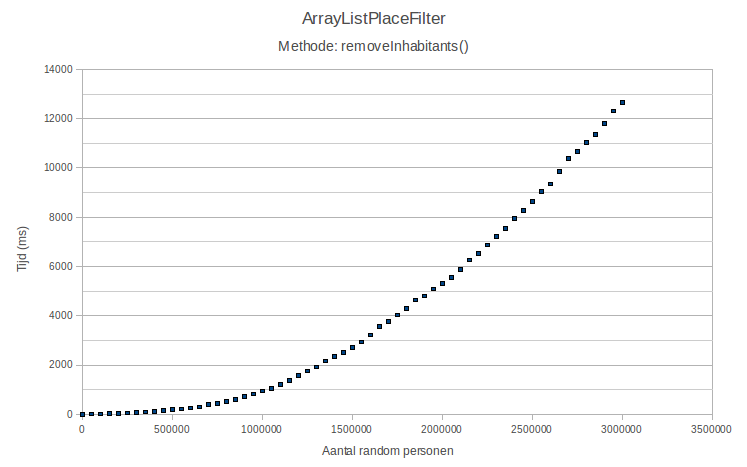
\includegraphics[width=0.84\textwidth]{ArrayListPlaceFilter:removeInhabitants.png}}
    \caption{ArrayListPlaceFilter.removeInhabitants()}
    \label{fig:ALPC-rI}
\end{figure}
\begin{figure}[h!]
    \centering
    \fbox{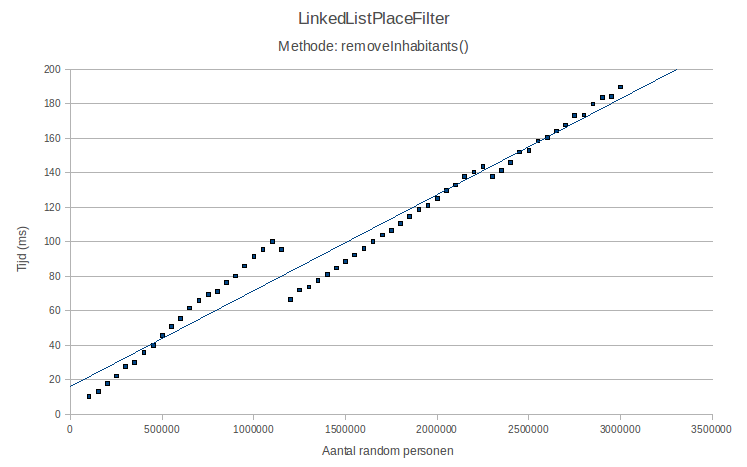
\includegraphics[width=0.84\textwidth]{LinkedListPlaceFilter:removeInhabitants.png}}
    \caption{LinkedListPlaceFilter.removeInhabitants()}
    \label{fig:LLPC-rI}
\end{figure}
\newpage
\subsubsection*{Bevindingen}
De grafieken gedragen zich inderdaad zoals ik had verwacht. Figuur \ref{fig:ALPC-rI} is duidelijk kwadratisch. Naar het eind stijgt hij minder en minder vlug. Dit komt omdat het 'opvullen' van de lege elementen steeds korter en korter duurt aangezien de lijst naar het eind kleiner en kleiner wordt.\\
Figuur \ref{fig:LLPC-rI} gedraagt zich ook duidelijk lineair, hoewel er wat vreemde dingen in zitten. Ik heb deze test een aantal keer herhaald en intussen mijn computer volledig opnieuw opgestart maar ik kreeg gelijksoortige grafieken. Ik gok dat dit een tussenkomst is van de JVM of van mijn CPU.

\subsection*{Welke datastructuur is volgens jou het meest geschikt?}
Uit de complexiteitsberekeningen en grafieken is het duidelijk dat een LinkedList het meest geschikt is.


%%%%%%%%%%%%%%%%%%%%%%%%%%%%%%%%%%%%%%%%%
%%%%			VRAAG 2              %%%%
%%%%%%%%%%%%%%%%%%%%%%%%%%%%%%%%%%%%%%%%%

\section*{Vraag 2: Frequenties van initialen}
\subsection*{Gebruikte datastructuren en algoritmen}
\subsubsection*{Gebruikte datastructuren}
Voor de eerste klasse, ListInitialsCounter, heb ik een ArrayList gebruikt. Het toevoegen bij een ArrayList is een geamortiseerde $\theta(1)$ aangezien hij soms zijn lijst moet kopieren. Bij een LinkedList is het ook $\theta(1)$. Het overlopen van beide lijsten is gelijk, namelijk $\theta(n)$ aangezien we hele lijst zouden moeten doorlopen. Het verwijderen is wel verschillend, maar aangezien we dit niet moesten doen heeft het geheugengebruik de doorslag gegeven. Bij een LinkedList wordt er namelijk 1 waarde en twee pointers opgeslagen, dit is niet het geval bij een ArrayList. Deze ArrayList is van het type String en bevat initialen van de voor- en familinamen van de personen.\\

Voor de tweede klasse werd er in de opdracht vermeld dat we van een HashMap gebruik moesten maken. Mijn HashMap heeft als Key een String waar de initialen worden opgeslagen. Als Value heeft mijn HashMap een integer wat het aantal voorkomens van die initialen zijn. 

\subsubsection*{Gebruik algoritme}
Het begin van de \textsl{addPerson()} methode van mijn twee klassen zijn gelijk. De voornaam en achternaam wordt steeds opgesplitst, waarna het eerste karakter van elk woord samengezet wordt. Dit geheel wordt dan enerzijds aan een ArrayList toegevoegd, of aan een HashMap. Bij mijn HashMap wordt er eerst gecontroleerd als de HashMap al een waarde voor die initialen bevat. Als dit het geval is telt hij 1 op bij het aantal voorkomens, anders wordt er een nieuwe Key en Value geplaatst met als Key de initialen en als Value 1.\\

De \textsl{getNrOccurences()} geeft bij het geval van een ArrayList het aantal voorkomens terug, berekend door de methode \textsl{frequency()} van de klasse Collections. In het geval van een HashMap gebruikt hij de methode \textsl{get()} om de integer terug te geven die bij de opgegeven initialen hoort.

\subsection*{Tijdscomplexiteit}
De \textsl{addPerson()} methode van ListInitialsCounter is geamortiseerd $\theta(1)$. Dit wil zeggen dat hij in praktijk gemiddeld $\theta(1)$ is, maar dat hij bij sommige waarden een complexiteit van $\theta(n)$ vertoond, namelijk op de momenten dat de lijst moet gekopieerd worden naar een nieuwe lijst om meer elementen te kunnen bevatten.\\
Bij de klasse HashMapInitialsCounter is de methode \textsl{addPerson()} ook constant, $\theta(1)$ dus, aangezien zowel de methode \textsl{containsKey()}, \textsl{get()} en \textsl{put()} hebben een complexiteit van $\theta(1)$.\\

De methode \textsl{getNrOccurences()} is echter wel verschillend. Bij een ArrayList zal hij van in het begin tot het eind de lijst overlopen. Dit zorgt ervoor dat we hier een complexiteit van $\theta(n)$ krijgen. Bij een HashMap hoeft hij enkel maar te getten op zijn Key, wat een complexiteit van $\theta(1)$ oplevert.

\subsection*{Tijdsmetingen}

\subsubsection*{Grafieken}
\begin{figure}[h!]
    \centering
    \fbox{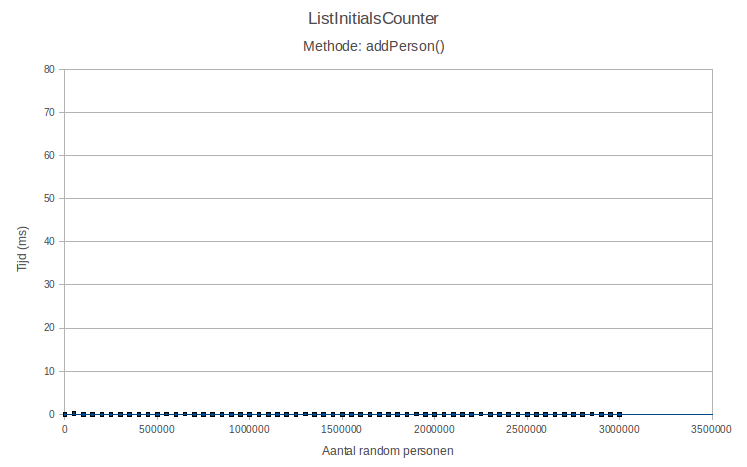
\includegraphics[width=0.83\textwidth]{ListInitialsCounter:addPerson.png}}
    \caption{ListInitialsCounter.addPerson()}
    \label{fig:LIC-aP}
\end{figure}
\begin{figure}[h!]
    \centering
    \fbox{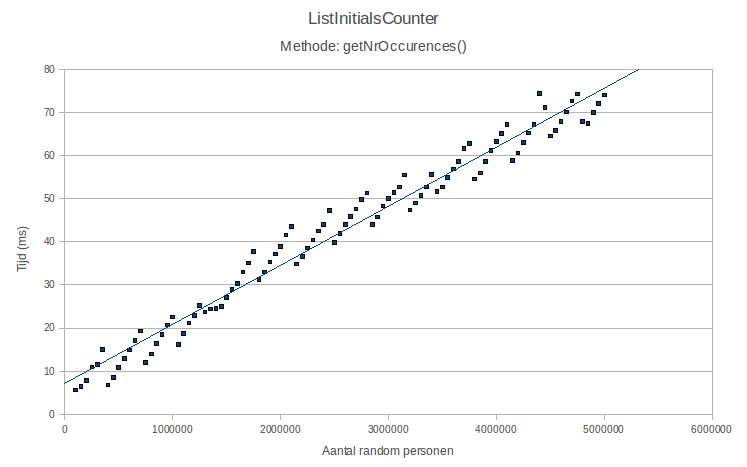
\includegraphics[width=0.83\textwidth]{ListInitialsCounter:getNrOccurences.png}}
    \caption{ListInitialsCounter.getNrOccurences()}
    \label{fig:LIC-gNO}
\end{figure}
\begin{figure}[h!]
    \centering
    \fbox{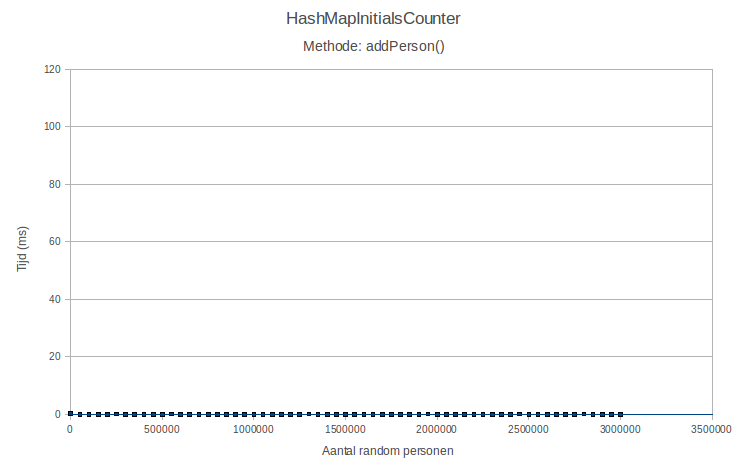
\includegraphics[width=0.83\textwidth]{HashMapInitialsCounter:addPerson.png}}
    \caption{HashMapInitialsCounter.addPerson()}
    \label{fig:HMIC-aP}
\end{figure}
\begin{figure}[h!]
    \centering
    \fbox{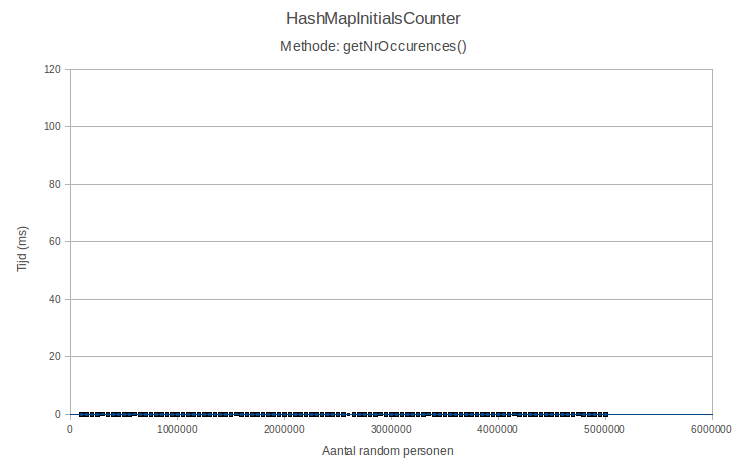
\includegraphics[width=0.83\textwidth]{HashMapInitialsCounter:getNrOccurences.png}}
    \caption{HashMapInitialsCounter.getNrOccurences()}
    \label{fig:HMIC-gNO}
\end{figure}
\newpage
\subsubsection*{Bevindingen}
Zoals verwacht gedragen beide datastructuren voor het invoegen van persoon zich constant. Dit tonen figuren \ref{fig:LIC-aP} en \ref{fig:HMIC-aP} nogmaals aan.\\
Ook bij de methode \textsl{getNrOccurences()} gedraagt de grafiek zich als verwacht zoals te zien is in figuren \ref{fig:HMIC-aP} en \ref{fig:HMIC-gNO}. Voor de ArrayList krijg ik min of meer een lineaire functie. Wat wel op valt is dat er steeds een stijging voor ongeveer 6 inputwaarden, waarna het even terugvalt in uitvoeringstijd. Ook deze test heb ik meerdere keren herhaald, met ongeveer dezelfde resultaten. Dit kan, zoals in Vraag 1 komen door de JVM, mijn CPU of garbage collection.

\subsection*{Welke datastructuur is volgens jou het meest geschikt?}
Zoals de berekeningen vooraf en de grafieken aantonen, is de beste datastructuur voor dit probleem een HashMap aangezien deze voor beide bewerkingen een complexiteit van $\theta(1)$ heeft.

%%%%%%%%%%%%%%%%%%%%%%%%%%%%%%%%%%%%%%%%%
%%%%			VRAAG 3                 %%%%
%%%%%%%%%%%%%%%%%%%%%%%%%%%%%%%%%%%%%%%%%

\section*{Vraag 3: Telefoonboek}
\subsection*{Gebruikte datastructuren en algoritmen}
\subsubsection*{Gebruikte datastructuren}
Als datastructuur heb ik hier gekozen voor een HashMap met als Key een persoon, meerbepaald MyPhonePerson, en als Value een ArrayList van Strings om de telefoonnummers bij te houden. De personen van het type MyPhonePerson worden eerst op gemeente, dan op naam en dan op voornaam gesorteerd. Ik heb deze datastructuur gekozen omdat je op deze manier gemakkelijk een telefoonnummer aan een peroon kan toevoegen en gemakkelijk telefoonnummers opvragen. Op deze manier is de \textsl{write()} methode relatief snel.

\subsubsection*{Gebruikte algoritmen}
In de methode \textsl{addPerson()} wordt eerst een nieuw MyPhonePerson aangemaakt. Vervolgens wordt op gekeken in de TreeMap als deze MyPhonePerson als Key bestaat. Als dit het geval is wordt er een nieuw telefoonnummer toegevoegd via de methode \textsl{addPhoneNumber()}. (De reden waarom ik dit doe is omdat anders de persoon overschreven wordt. Als we dit op een andere manier zouden doen, bijvoorbeeld om te kijken als het ID van de persoon al bestaat of niet, zou dit later problemen oplever bij de methode \textsc{•}f{getNumbers()}. Hij zou dan namelijk de nummers van meerdere personen teruggeven, wat niet de bedoeling is.) Als de persoon nog niet bestaat voegt hij deze in de TreeMap met als Key de objectreferentie naar de persoon, en als Value een ArrayList met zijn telefoonnummer.\\

Bij de methode \textsl{getNumbers()} maakt hij een nieuw persoon aan met de opgegeven waarde om zo de lijst van telefoonnummers te kunnen teruggeven.\\

De methode \textsl{addPhoneNumber()} maakt eerst een nieuw persoon aan. Hij controleert eerst als de persoon waar het telefoonnummer erbij moet toegevoegd worden er wel degelijk in zit om NullPointerExceptions te vermijden. Daarna wordt de lijst van telefoonnummers werkelijk uit de TreeMap gehaald en wordt het opgegeven telefoonnummer eraan toegevoegd.\\

De methode \textsl{write()} bestaat uit een for-each loop die itereert over de Keys van de TreeMap. Per Key maakt hij een StringBuilder aan die enkele gegevens uitprint. Na het uitprinten van de gegevens itereert hij over de ArrayList die hij ophaalt met de \textsl{get()} methode. Uiteindelijk print hij alles uit naar de terminal.

\subsection*{Tijdscomplexiteit}
Aangezien de methode \textsl{addPerson()} gebruikt maakt van de \textsl{addPhoneNumber()} zal ik eerst de complexiteit van de laatste methode bespreken.\\
De methode \textsl{addPhoneNumber()} maakt eerst gebruik van de \textsl{containsKey()} methode. Volgens de Java documentatie is deze gegarandeerd $\theta(log(n))$. Daarna haalt hij de lijst van telefoonnummers op via de \textsl{get()} methode. Ook dit heeft als complexiteit $\theta(log(n))$. Uiteindelijk voegt hij het opgegeven telefoonnummer toe aan de lijst van telefoonnummers. Dit laatste is een geamortiseerde constante, $\theta(1)$ dus. De samenstelling van deze functies geeft ons $\theta(log(n))+\theta(log(n))$, wat herleid wordt naar $\theta(log(n))$.\\

De methode \textsl{addPerson()} heeft twee mogelijkheden: Of de persoon bestaat al. Hierbij maakt hij gebruik van de methode \textsl{addPhoneNumber()}, waarvan de complexiteit in de vorige paragraaf al besproken werd. De andere mogelijkheid is dat de persoon nog niet bestaat. In dit laatste geval voegt hij een String via de methode \textsl{add()} toe aan een ArrayList. Dit is een geamortiseerde constante, complexiteit $\theta(1)$ dus. Hierna maakt hij gebruik van de methode \textsl{put()}. Dit laatste heeft volgens de Java documentatie een complexiteit van $\theta(log(n))$.\\

De methode \textsl{getNumbers()} haalt een waarde uit een TreeMap met de methode \textsl{get()}. Dit heeft volgens de Java documentantie een complexiteit van $\theta(log(n))$.\\

De methode \textsl{write()} maakt gebruik van een for-each iteratie om het telefoonboek op te bouwen. In deze for-each zit nog een for-each lus om de telefoonnummers uit te schrijven, maar deze is onafhankelijk van de grootte van de TreeMap. Er kan wel gezegd worden dat deze waarde verwaarloosbaar is ten opzichte van de grootte van de TreeMap. Om deze reden zal ik deze dan ook als een constante behandelen. Er kan besloten worden dat de totale complixiteit $\theta(nlog(n))$ zal zijn.

%%%%%%%%%%%%%%%%%%%%%%%%%%%%%%%%%%%%%%%%%
%%%%			VRAAG 4                 %%%%
%%%%%%%%%%%%%%%%%%%%%%%%%%%%%%%%%%%%%%%%%

\section*{Vraag 4: Oudste inwoner}
\subsection*{Gebruikte datastructuren en algoritmen}
\subsubsection*{Gebruikte datastructuren}
Als datastructuur heb ik een TreeMap gebruikt met als Key een String, namelijk de naam van de gemeente, en als value een TreeSet van personen, meerbepaald van MyOldestPerson. De personen van het type MyOldestPerson worden eerst op leeftijd gesorteerd, dan op naam en dan op voornaam.\\
Ik heb voor deze structuur gekozen zodat ik makkelijk een lijst kan halen uit mijn TreeMap op basis van de ingegeven gemeente en daarover kan itereren om de oudste n aantal personen terug te geven. Dit natuurlijk met het oog op de korst mogelijkste uitvoeringstijd.

\subsubsection*{Gebruikte algoritmen}
De methode \textsl{addPerson()} maakt eerst een tijdelijke TreeSet met als type MyOldestPerson aan. Daarna kijkt hij als de gemeente van de opgegeven persoon al voor komt in de HashMap. Als dit het geval is haalt hij de lijst via de \textsl{get()} methode uit de HashMap en kent hij deze toe aan de TreeSet. Anders maakt hij een nieuwe TreeSet aan. Vervolgens wordt de persoon toegevoegd aan de lijst via de \textsl{add()} methode en wordt de lijst met de juiste Key terug in de HashMap gestopt via de methode \textsl{put()}.\\

De methode \textsl{findOldestPeople()()} overloopt de personen gesorteerd op leeftijd die bij een gemeente horen. Iedere keer hij een persoon toevoegt gaat er een teller omhoog. Als het maximaal aantal terug te geven personen nog niet overschreden is, met andere woorden: als de teller kleiner is dan het aantal gevraagd personen, voegt hij het ID van de persoon toe aan de terug te geven lijst. Hij houdt ook de leeftijd bij van de minst jonge terug te geven persoon zodat bij een ex eaquo de personen terug gegeven worden waarvan hun leeftijd hetzelfde is als de laatst terug te geven persoon zijn leeftijd is. Als uiteindelijk het aantal terug te geven personen overschreden is, en de leeftijd van de huidige persoon komt niet meer overeen met de jongste terug te geven persoon wordt de lus afgebroken. Als het aantal gevraagde personen groter is dan het aantal personen in de lijst zal hij gewoonweg alles overlopen en alle personen van die gemeente terug geven, zoals in de opgave gevraagd wordt.

\subsection*{Tijdscomplexiteit}
De methode \textsl{addPerson()} maakt eerst gebruik van de methode \textsl{containsKey()} van een HashMap. Deze heeft als complexiteit $\theta(1)$. De methode \textsl{get()} heeft ook als complexiteit $\theta(1)$. De volgende methode is anders. Aangezien de grootte van de TreeSet niet afhankelijk is van de grootte van de HashMap moeten we hier een andere functie voor gebruiken. In plaats van $n$ zal ik hier $m$ gebruiken. Het toevoegen aan een TreeSet heeft volgens de Java documentatie $\theta(log(m))$ als complexiteit. Het toevoegen aan een HashMap is dan weer $\theta(1)$. We kunnen besluiten dat deze functie als complexiteit $\theta(log(m))$ heeft.\\

De methode \textsl{findOldestPeople()()} maakt eerst van de methode \textsl{get()} gebruik om de TreeSet met personen van de opgegeven gemeente te halen. Dit heeft als complexiteit $\theta(1)$. Daarna wordt ge\"itereerd over de personen, maar aangezien dit niet noodzakelijk afhankelijk is van het aantal random personen brengt dit een complexiteit van $\theta(n)$ met zich mee. Dit algoritme zou dus een complexiteit van $\theta(m)$ hebben.
\newpage
\subsection*{Tijdsmetingen}
\subsubsection*{ }
\begin{figure}[h!]
    \centering
    \fbox{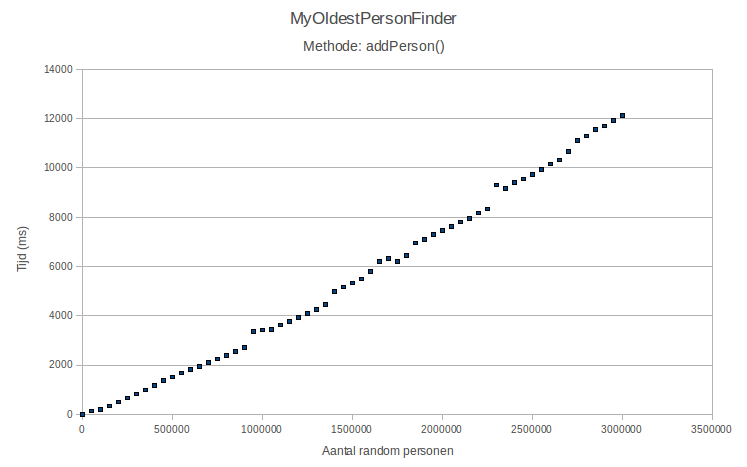
\includegraphics[width=0.9\textwidth]{MyOldestPeopleFinder:addPerson.png}}
    \caption{MyOldestPeopleFinder.addPerson()}
    \label{fig:MOPF-aP}
\end{figure}
\begin{figure}[b!]
    \centering
    \fbox{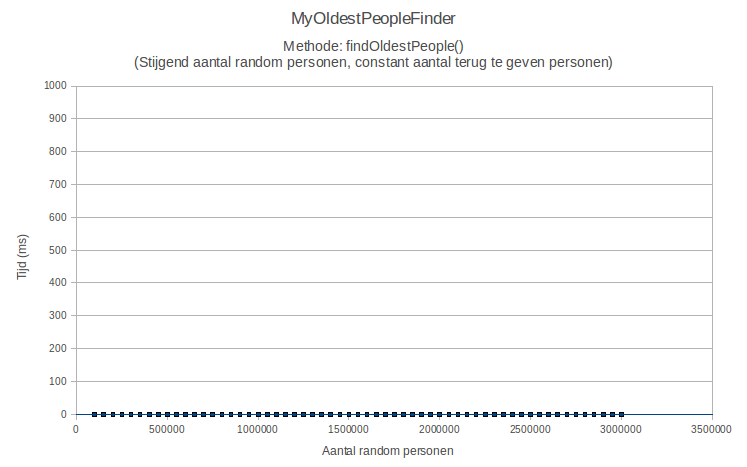
\includegraphics[width=0.9\textwidth]{MyOldestPeopleFinder:findOldestPeople1.png}}
    \caption{MyOldestPeopleFinder.findOldestPeople().1}
    \label{fig:MOPF-fOP1}
\end{figure}

Figuur \ref{fig:MOPF-aP}: Deze tijdsmeting meet hoelang het duurt om reeks personen toe te voegen. Hij lijkt op het eerste zicht lineair. Het is echter verwonderlijk dat je zo'n grote waarden zou krijgen met een lineaire functie.  In het boek, echter, staat op p. 46 vermeld dat er in de praktijk geen groot verschil is tussen een $\theta(n(log(n))$ algoritme en een $\theta(n)$ algoritme. We mogen er dus van uit gaan dat dit klopt met mijn oorspronkelijke bevindingen.


\begin{figure}[h!]
    \centering
    \fbox{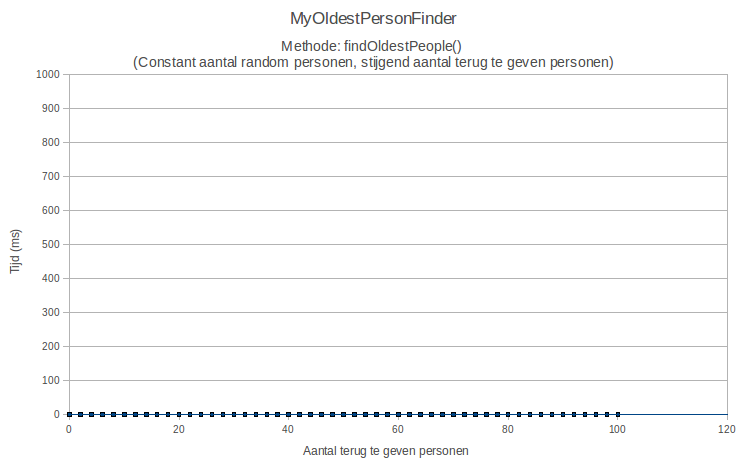
\includegraphics[width=0.80\textwidth]{MyOldestPeopleFinder:findOldestPeople2.png}}
    \caption{MyOldestPeopleFinder.findOldestPeople().2}
    \label{fig:MOPF-fOP2}
\end{figure}
\begin{figure}[h!]
    \centering
    \fbox{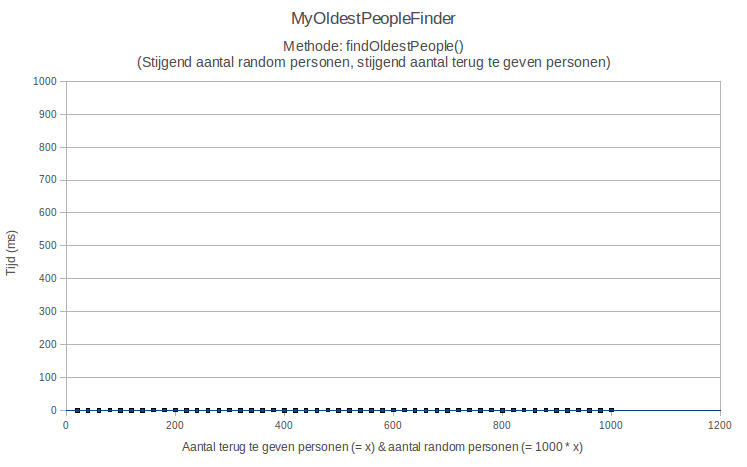
\includegraphics[width=0.80\textwidth]{MyOldestPeopleFinder:findOldestPeople3.png}}
    \caption{MyOldestPeopleFinder.findOldestPeople().3}
    \label{fig:MOPF-fOP3}
\end{figure}

Om de methode \textsl{findOldestPeople()} te testen heb ik drie verschillende testen gedaan. Ik heb het algoritme eerst laten zoeken in een HashMap met een stijgend aantal random personen en een constant aantal terug te geven personen (figuur \ref{fig:MOPF-fOP3}). Daarna met een constant aantal personen en een stijgend aantal terug te geven personen (figuur \ref{fig:MOPF-fOP2}) en als laatste met een stijgend aantal random personen en een stijgend aantal terug te geven personen (figuur \ref{fig:MOPF-fOP3}). Mijn resultaten komen wel niet overeen met de theoretische berekeningen. Een mogelijke verklaring kan zijn dat ik met hogere inputwaarden moest werken om een beter beeld te krijgen van hoe de functie zich verder ontwikkelt.

\end{document}